\documentclass[12pt]{extarticle}
\usepackage{tikz}
\usetikzlibrary{calc}
\usepackage{eso-pic}
\usepackage{datetime}
\usepackage{lipsum}
\usepackage{graphicx}
\graphicspath{ {/home/pratik/Desktop}}
\AddToShipoutPictureBG{%
\begin{tikzpicture}[overlay,remember picture]
\draw[line width=6pt]
    ($ (current page.north west) + (0.8cm,-0.8cm) $)
    rectangle
    ($ (current page.south east) + (-0.8cm,0.8cm) $);
\draw[line width=1.5pt]
    ($ (current page.north west) + (1.2cm,-1.2cm) $)
    rectangle
    ($ (current page.south east) + (-1.2cm,1.2cm) $);
\end{tikzpicture}
}
\usepackage{color}
\date{}
\author{\textbf{Vaibhav Vashisht} 2016CSJ0002  \\\textbf{Pratik Parmar} 2016CSJ0049}
\title{\textbf{COP290: Design Practices\\ Software Requirement Document \\ AC Circuit Solver  }}
\begin{document}
\maketitle
\newpage

%\begin{center}
%\section*{\underline{\textbf{AC Circuit Solver}}}
%\end{center}

\section{Introduction}

\subsection{Purpose}
The purpose of this application is to build an application for drawing electrical circuits and solve them.
\subsection{Document Conventions}
\textbf{Netlist:} Connectivity of circuit in terms of nets. For eg
0 is always grounded.\\
\\R1 Net1 0 10K\\
C1 Net0 Net1 100NF\\
L1 Net0 0 10NH\\
R2 Net0 0 1K\\
C2 Net0 0 10NF\\
I1 Net0 0 SINE ( 0 1 10Khz 0.0S 0 )\\ \\This represents R1 is a resistor connected b/w Net1 and 0(ground) of 
10K Ohms,same logic follows for other elements described.An image of the circuit described by the above netlist is given below:\\
\\
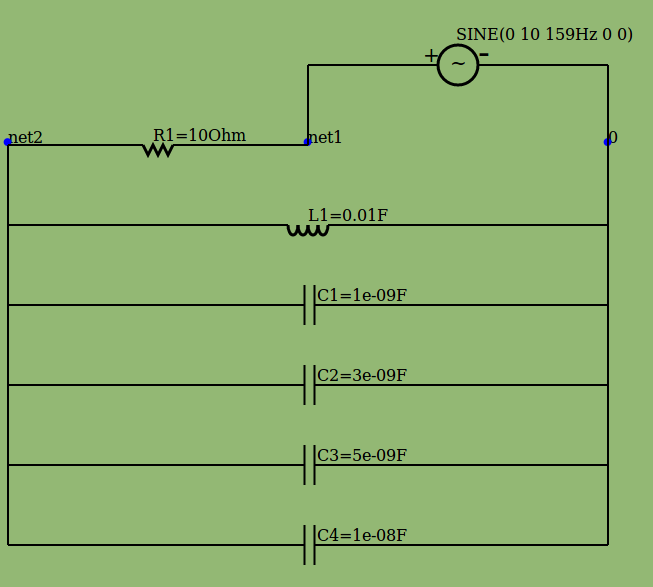
\includegraphics[width=14cm, height=8cm]{Top}
\section{Project Scope}
The purpose of this project is to simplify circuit analysis.Scientists sometimes require results of a given circuit for research purpose,this project would simplify their work as they need not do in depth analysis of that circuit but can use the results directly.
\section{Product Features}
As already mentioned this application extracts the circuit user wants to draw in terms of netlist and renders the circuit as an SVG image.\\ The user is able perform the following features-:
\begin{enumerate}
\item Zoom image as per convenience
\item Draw a circuit with large number  of nodes as large as 1000 or more.
\item \textbf{Clickable components}- User can click on resistor,capacitor or any other circuit component and obtain the stats of the corresponding elements i.e voltage across it,current flowing through it etc.
\item \textbf{Detect Circuits}- If a user wants to check whether the circuit given by the netlist is valid or not,it can be done easily by giving the netlist corresponding  to that circuit as an input to the application ,which will display invalid circuit message in case the circuit is not valid and draw the circuit if its valid. 
\end{enumerate}
\section{Operating Environment}
AC circuit Solver would work on a Linux based operating system with all the required Software/Packages installed on it.
\newpage
\section{Software Requirement}
Following Software/Packages are Required for running this application.
\begin{enumerate}
\item Linux Based Operating System preferably Ubuntu
\item GNU g++ Compiler for C++
\item Flex(Fast Lexical Analyser Generator)
\item Bison
\item HTML Viewer or Web Browser(Firefox or Chrome)
\end{enumerate}

\section{Technical Process}
Following would be the Languages/tools would be used to develop this application
\begin{enumerate}
\item Functionality: C++
\item Image Rendering: SVG
\item Interactivity in Image: JavaScript
\item Styling: CSS
\item Layout: HTML and XML
\item Scripting: Bash
\item Automation: Python
\end{enumerate}

\section{Software Quality Attributes}
\begin{enumerate}
\item \textbf{Display:} The application should display the correct circuit as described by the netlist.
\item \textbf{Correctness:} The output file containing the correct voltage and current values across each component.
\item \textbf{Clickable:} One should be able to click any element of the circuit and view it and its properties separetly.

\end{enumerate}

\end{document}

